
\medskip  

%C'est en 1891 que les premiers vietnamiens arrivèrent en Nouvelle-Calédonie pour travailler dans les mines de nickel. De nos jours, leurs descendants continuent à transmettre leur héritage au travers de manifestations culturelles. 
%
%Un des symboles de cet héritage est celui du \og N\'on l\'a \fg{} communément appelé chapeau chinois dont une image est donnée ci-dessous. On considère que ce chapeau est un cône. 
%
%\parbox{0.65\linewidth}{
%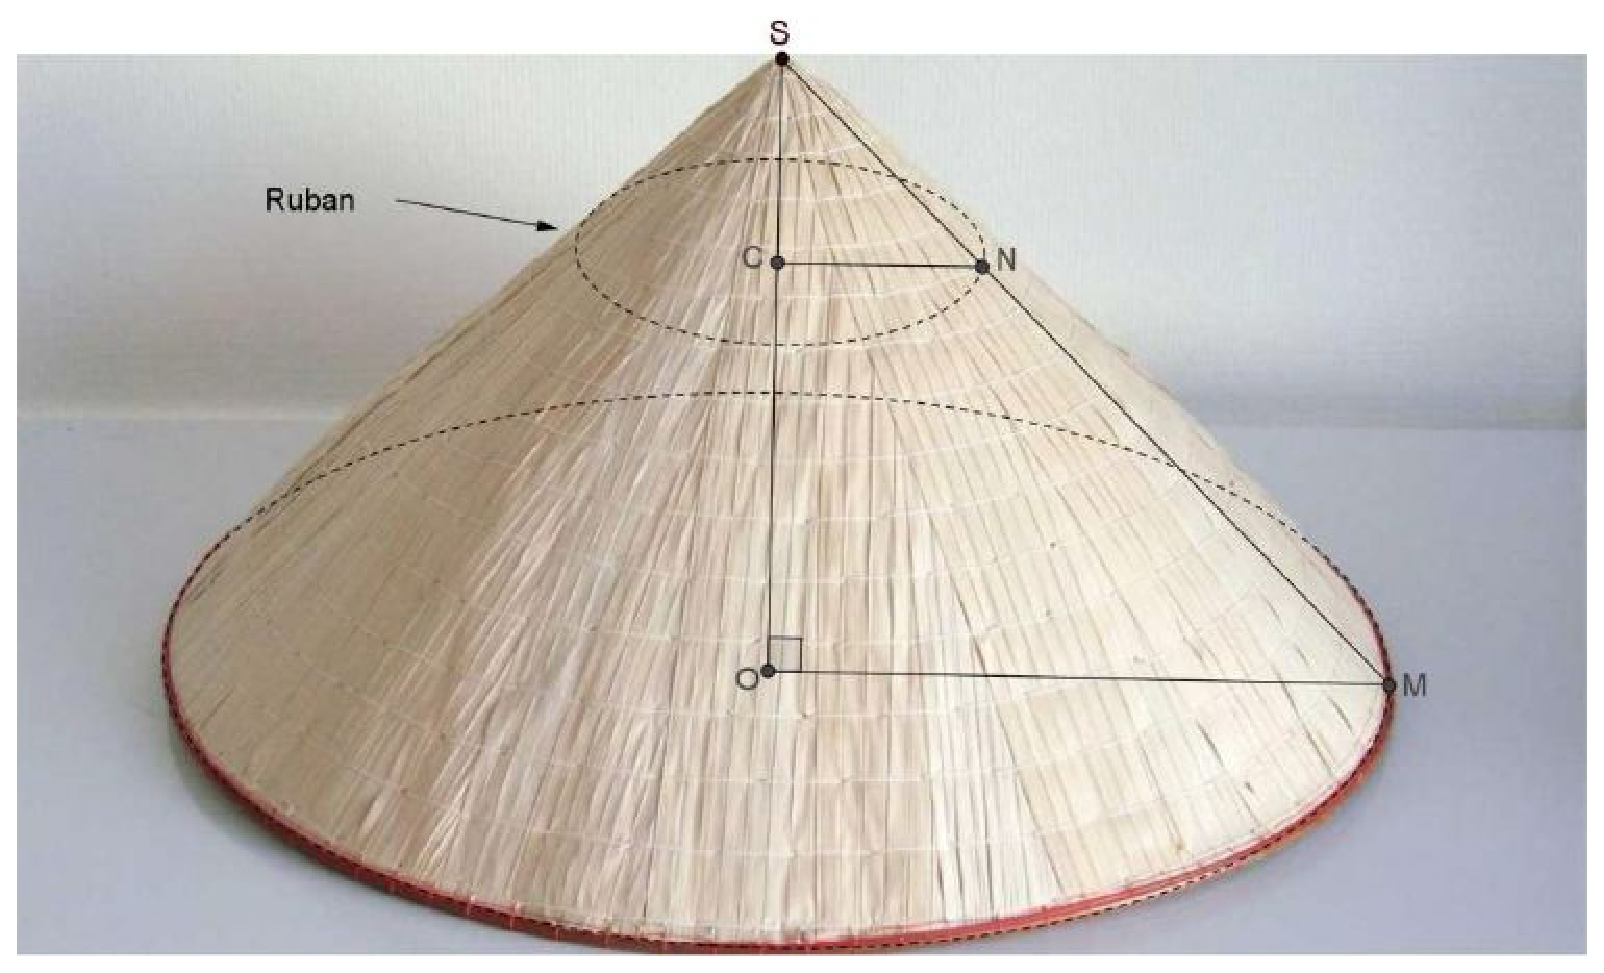
\includegraphics[width=.65\textwidth]{chapeauchinois.eps}}\hfill\parbox{0.3\linewidth}{Données : 
%
%SOM est rectangle en O 
%
%OM = 24 cm 
%
%SM = 37,5 cm.}
%
%\medskip
 
\begin{enumerate}
\item %Calculer la hauteur SO, arrondir à l'unité. 
Dans le triangle SOM rectangle en O, le théorème de Pythagore permet d'écrire :

$\text{SM}^2 = \text{SO}^2 + \text{OM}^2$, soit $\text{SO}^2 = \text{SM}^2 - \text{OM}^2 = 37,5^2 - 24^2 = 830,25$.

Donc SO $ = \sqrt{830,25} \approx 28,8$ donc 29 cm à l'unité près.
\item %En guise de décoration, on se propose de poser un ruban autour du chapeau parallèlement à sa base. 

%Ce ruban est disposé au \textbf{tiers} du chapeau en partant du sommet. 
	\begin{enumerate}
		\item %Quelle est la nature de la figure géométrique formée par ce ruban ?
Le ruban prendra la forme d'un cercle. 
		\item %Calculer en cm la longueur du ruban.
Le rayon du cercle précédent est le tiers de celui du chapeau OM soit 

$\dfrac{1}{3} \times 24 = 8$~cm.
		
La longueur du raban est donc : $16\pi \approx 25$~cm. 
	\end{enumerate}
%Toute trace de recherche, même incomplète ou non fructueuse, sera prise en compte dans l'évaluation de cet exercice. 
\end{enumerate}

\vspace{0,5cm}

